
\documentclass{article}

\usepackage{fullpage}

\usepackage{color}

\usepackage{amsmath}

\usepackage{textcomp}
\usepackage{ifthen}
\usepackage{listings}
\usepackage{fancyvrb}
\usepackage{verbatim}
%\usepackage[noend]{algorithm2e}

%\usepackage[pdftex]{graphicx}
\usepackage{graphicx}
%\usepackage{subfig}
\usepackage{calc}
\usepackage{float}
\usepackage{caption}
\usepackage{subcaption}

\usepackage{url}

% For generating custom lists (similar to table of contents, list of figures
% etc.)
\usepackage[subfigure]{tocloft}

\usepackage{hyperref}
\usepackage[all]{hypcap}
\usepackage{latexsym}

\usepackage{enumitem}

% Remove spacing around section headings
\usepackage[compact]{titlesec}
\titlespacing{\section}{0pt}{*0}{*0}
\titlespacing{\subsection}{0pt}{*0}{*0}
\titlespacing{\subsubsection}{0pt}{*0}{*0}

%\usepackage[left=1.05in,right=1.05in,top=1in,bottom=1in]{geometry}

% tweak or comment out the baselinestretch to control how much space for hand-writing comments you get between the lines
%\renewcommand{\baselinestretch}{1.8}

%\newcommand{\reminder}[1]{}
\newcommand{\reminder}[1]{ [[[ \marginpar{\mbox{$<==$}} #1 ]]] }
%\newcommand{\yoav}[1]{\reminder{#1}}
%\newcommand{\reminder}[1]{
%    \par
%    \colorbox[rgb]{0.8,0.8,0.8}{
%        \parbox{\linewidth}{
%            #1
%        }}}
%\renewcommand{\reminder}[1]{}

\newcommand{\eat}[1]{}

\newtheorem{defin}{Definition}[section]
\newtheorem{ex}{EXAMPLE}[section]
%\newtheorem{lemm}{Lemma}[section]
%\newtheorem{thm}{Theorem}[section]
\newenvironment{example}{\begin{ex} \nopagebreak
  \begin{rm}}{\end{rm} $\Box$ \end{ex}}
%\newenvironment{definition}[1]{\begin{defin}\begin{rm}({\bf
%    #1})}{{\hfill$\Box$}\end{rm}\end{defin}}
%\newenvironment{lemma}{\begin{lemm}}{{\hfill$\Box$}\end{lemm}}
%\newenvironment{theorem}{\begin{thm} \nopagebreak}{{\hfill$\Box$}\end{thm}}


% Commands for writing syntax
\newcommand{\gn}[1]{{\bf #1}}       % (N)on-terminal
\newcommand{\gt}[1]{{\tt #1}}       % (T)erminal
\newcommand{\gs}[1]{{\it #1}}       % (S)pecial construct

% Verbatim environment for SQL snippets
\DefineVerbatimEnvironment% 
{sql}{Verbatim}{frame=single,numbers=left,fontsize=\scriptsize}

% HACK: Bypass ACM's definition of paragraph as a subsubsection
\renewcommand{\paragraph}[1]{{\noindent {\bf #1}}}

% Compress whitespace around itemize and enumerate
\setitemize{topsep=.0em,parsep=0pt,partopsep=0pt,labelsep=0.2em,itemsep=0pt,leftmargin=0.5em}
\setenumerate{topsep=.0em,parsep=0pt,partopsep=0pt,labelsep=0.2em,itemsep=0pt,leftmargin=0.5em}

% Remove paragraph indentation
\setlength{\parindent}{0pt}

% Remove paragraph spacing
\setlength{\parskip}{0pt}
\setlength{\parsep}{0pt}
\setlength{\headsep}{0pt}
\setlength{\topskip}{0pt}
\setlength{\topmargin}{0pt}
\setlength{\topsep}{0pt}
\setlength{\partopsep}{0pt}

% Decrease the line spread slightly
% \linespread{0.98}

% Define our own compact enumerate
%\newenvironment{compact_enum}
%{\setlength{\leftmargini}{1em}
%\begin{enumerate}
%  \setlength{\labelsep}{.3em} 
%  \setlength{\itemsep}{.4em}
%  \setlength{\parskip}{0pt}
%  \setlength{\parsep}{0pt}}
%{\end{enumerate}}

% Define our own compact itemize
%\newenvironment{compact_item}
%{\setlength{\leftmargini}{1em}
%\begin{itemize}
%  \setlength{\labelsep}{.3em} 
%  \setlength{\itemsep}{.4em}
%  \setlength{\parskip}{0pt}
%  \setlength{\parsep}{0pt}}
%{\end{itemize}}

%\addtolength{\topmargin}{-8mm}
%\addtolength{\topskip}{-1mm}

\DefineVerbatimEnvironment%
{tree}{Verbatim}{frame=single,fontsize=\scriptsize}

\DefineVerbatimEnvironment%
{treeNumber}{Verbatim}{frame=single,numbers=left,fontsize=\scriptsize}
\title{Data-driven workflow application frameworks for mobile}

\renewcommand{\rmdefault}{phv} % Arial
\renewcommand{\sfdefault}{phv} % Arial

\begin{document}

\section{Introduction}
\label{sec:introduction}
Since the 80s, SQL database systems gradually became the foundation of Business Intelligence (BI) and On Line Analytical Processing (OLAP) applications. Their success is primarily attributed to {\em declarative querying} (via SQL), {\em automatic query optimization} and {\em physical-logical independence}, which are explained in Section~\ref{sec:healthy-aspects}. These healthy features of SQL led to increased developer and analyst productivity. They also led to specialized roles for the participants, whereas each participant (database developer, database administrator) needs to master only one layer of the overall architecture. 

However, SQL systems fail in the space of predictive analytics that involve sensors generating measurements in the space and time dimensions.%
\footnote{Indeed, one may argue that some of the discussed failures and respective remedies proposed by Plato, also apply to predictive analytics of non-sensor, non-spatiotemporal data. Nevertheless, the focus of this project is exclusively on spatiotemporal sensor data.
}
Section~\ref{sec:the-failure} argues that at the core of the failure of SQL databases in the management and analytics of sensor spatiotemporal data is the lack of a critical abstraction, which is the {\em real world model}, which captures a stochastic process that generates the measurements.%
\footnote{The real world model is frequently called the ``physical model" as it corresponds to the physics of the real world. This proposal uses the term ``real world model" (instead of the term ``physical model") to avoid the confusion caused by the two different meanings of the word ``physical" in the sensors' signal processing and the database community.
}

The signal processing area has deeply built in its foundations the real world model concept, which leads to great results in the cleaning, compression and reconstruction of signals. However, this area's approaches have been directly applicable only to problems with (a) low diversity of data (e.g., when the entire data set of interest comes from a single type of sensor and there are no ``metadata" and/or other alphanumeric data to provide context to the sensor data analysis and its results), (b) low volume of data, with no complex needs on how to effectively persist the data set over time and (c) a single type of ``hardwired" analysis. 
% Furthermore they require highly knowledgeable signal processing experts, who must combine statistics.
It is apparent that databases and signal processing techniques should be coupled but, unfortunately, currently they do not mix well. The result is reduced productivity, very high requirements on the analysts (must be simoultaneously experts in signal processing, statistics and big data management) and projects that cannot easily incorporate many types of data and many types of analysis.

\reminder{to Yannis P: fix the roadmap}

Section~\ref{sec:plato} introduces the proposed Plato database system, which brings the real world model concept into SQL databases, therefore combining the healthy productivity aspects of SQL systems (declarative queries, multiple levels of abstraction, automated optimization) with the sensor data processing benefits of signal processing techniques.

Section~\ref{sec:noise-reducted} argues that the noise-reducted, additive models that can be derived from common learning algorithms (in the field of signal processing) confer both a data quality benefit and a huge efficiency benefit, by virtue of providing very compressed representations of the model. Query processing algorithms can run directly on these compressed representations.

% Incremental maintenance
%Section~\ref{sec:} ....


\subsection{The healthy aspects of SQL databases in analytics}
\label{sec:healthy-aspects}
In a typical database-driven application architecture (see Figure~\ref{fig:db-driven-arch}), the business intelligence application issues an SQL query over tables. As far as the application is concerned, the tables are {\em logical} in the sense that they are just mathematical relations. In contrast, the underlying data structures where the tables are stored, as well as the indices on the tables, constitute the {\em physical} layer, whose knowledge is not needed for writing queries. The queries are declarative in the sense that they only describe the desired result without describing the algorithm that computes the result. A query optimizer automatically finds a good plan (in effect, algorithm) for executing the query, taking into consideration the specifics of the physical layer. Declarativeness and automatic optimization increase {\em developer productivity} and {\em lower the sophistication bar} needed for writing analytics. Furthermore, they are a key enabler behind visual OLAP systems, where the (non-programming) user can easily aggregate, correlate, drill-down in the data, pivot, etc. During runtime, such systems (e.g., Cognos, Microstrategy) face the relatively easy task of translating clicks into declarative queries, while the problem of optimizing these queries is left to the database.

A database administrator may ``tune" the physical layer from time to time in order to boost the performance of the observed workload. However, logical/physical separation says that such tuning changes at the physical layer do not require rewriting of the logical layer. Rather, the query processing speed automatically benefits. Notice how logical/physical separation divides the expertise and tasks needed for the maintenance of the overall system, therefore making its maintenance and evolution very easy and inexpensive.

Further levels of abstraction are achieved with {\em views}, which are tables that capture the result of filtering, combining and aggregating the data of the logical tables in a way that simplifies the queries issued by the applications. A database administrator may elect to materialize some views, in order to precompute some of the computations that the live queries must perform. Again, notice that when the database administrator changes a view from virtual to materialized, the developer need not change her queries.

\begin{figure}
{\bf the conventional database-driven analytics architecture illustrating declarative query and optimizer that automatically finds how to utilize the data structures best.}
\caption{Database-driven analytics architecture}
\label{fig:db-driven-arch}
\end{figure}

\subsection{The failure of SQL databases in spatiotemporal sensor data analytics}
\label{sec:the-failure}
In conventional SQL databases, the data contained in the database have a one-to-one mapping to the captured real world objects and events. For example, a database may represent persons, which have an address, a name and a telephone number. Each represented person is supposed to be a corresponding unique entity in the world. Vice versa, as far as the database and the applications running on it are concerned, the represented entities, attributes and relationships constitute the entire real world of interest. In contrast to a conventional database, the sensor data are mere {\em measurements} (samples) of the reality. The full reality of interest to the analytics application is captured by models that predict the quantity of interest at each point in a range of time and/or space. In practice, the gap between the measurements and the real world models is best crossed by learning algorithms that discover the parameters of the real world model and are tuned to the type of the model. For example, when one models a temporal signal exhibiting periodicity, she will use the Fourier transform to discover the frequencies. Given the frequencies, the model can predict a value for any time.

A second cornerstone of statistical sensor data processing, also missed by SQL systems, is the assumption that the real world process that leads to the measurements is a stochastic process. Respectively, an issued query may not return a single predicted value for a quantity; rather, it should return a probability distribution for the predicted value, often simplified by providing an expected value and a confidence interval.

In the absence of real world models in database systems, various suboptimal approaches are used. An approach is to use a database simply as a ``dumb" storage of measurements. Then
given an analytics request, one has to first issue queries that retrieve the relevant measurements. Then she deploys signal processing learning algorithms on them to compute the model's parameters. Finally,  the results are moved into the database. In a variation to this approach, one may not use a SQL database at all (since SQL does not buy her significant functionality anyway) and instead rely on file systems (including the highly scalable distributed file systems). 

In either case, the healthy aspects of SQL database systems discussed in Section~\ref{sec:healthy-aspects} are no longer observed. Instead, the above process is characterized by low productivity as data move in an out of the database in hardwired ways. The approach does not scale to cases with high diversity of data (e.g., when there are ``metadata" and/or other alphanumeric data that provide context to the sensor data analysis and its results) and the analytics application may issue multiple types of  requests. Furthermore, unlike the ecosystem of conventional SQL systems, the analysts of sensor data must be experts of many areas: signal processing, statistics, databases and often big data management and processing. As sensor data proliferate, the short supply of such multiarea experts and the low productivity in developing and maintaining sensor analytics will lead to a world where a lot of sensor data will be collected but only limited analysis will be performed at them, at the cost of missing the insights that these data can offer.

% In a second approach, one may trivialize . For example, This approach can suffer from quality issues and/or performance issues. First, unless the set of measurements is very dense there is a risk that the interpolated values 

In recent years databases have been extended (typically via UDFs) with machine learning procedures that can allow one to execute such procedures without moving data in-and-out of the database. While such extensions are useful, we argue next that they miss the optimization opportunities that become available once models appear in the database as first class citizens and the query language and query processing are adjusted accordingly. Furthermore, they do not account yet for the probabilistic nature of the data and the statistical nature of the queries.

Recent research systems have expanded SQL databases to probabilistic facts (as opposed to the conventional merely boolean facts). As we discuss next, the proposed system assumes that the models are also associated with probabilities.

%The net effect is that analytics on spatiotemporal sensor data currently require the involvement of developers who are essentially skilled in all of the (a) data filtering and combining, (b) modeling, and (c) low level data representation and related algorithms. 
% the decoupling shown earlier has collapsed.

\subsection{Plato: Models as a first class citizen of the database and query language}
\label{sec:plato}
The proposed Plato database has models as a ``first class citizen" abstract type of the database. If we neglect the stochastic aspect of the data, a Plato model is a continous function over time and/or space that predicts a quantity of interest (eg, temperature, velocity, acceleration, air pollutants density etc) at any coordinate in a certain time/space area. Alternately, a database-minded person may perceive a Plato model as a table whose attributes are time and/or space coordinates and one or more types of quantities. The table has infinitely many tuples and the time/space coordinates form a key, i.e.,  given values for the time/space coordinates, each quantity has a unique associated value. 
In order to capture the stochastic aspect of a process, Plato further assumes that the process may be described by multiple functions, where each function is assigned a probability.

% Queries that one can write.
% Challenge: develop the query languages

Consequently, Plato expands the applicability of the successful architecture of Figure~\ref{fig:db-driven-arch} into statistical, spatiotemporal sensor data management and analytics. The application issues declarative ``Plato SQL" queries, which utilize the models without being concerned about the specifics of how the models are actually represented in the storage nor the intricacies of how to most efficiently execute the queries. (Representation in storage and efficient query execution is introduced next, in Section~\ref{sec:reduced-noise-additive}). \reminder{to YK: place section reference. Check whether these are still the examples we have. I do not mind switching the following to the examples you wrote.} Section~\ref{sec:} provide multiple examples of Plato SQL queries. In one example, a query predicts quantities at specific coordinates; in the stochastic counterpart of the example, the query also asks for the confidence interval, given pi value 0.05. In another example, models are correlated. In a third example, queries drill into specific time segments of the models; e,g., the afternoon times. In yet another example, models capturing the daily paths of individual persons are composed with models that provide the distribution of atmospheric polutants in San Diego County and the result is models of the polutant levels that these persons breathed; the query that composes the models is essentially just a simple SQL join. These model-related queries are seamlessly combined with the rest of the database, therefore making it easy to draw results about various segments of the entities represented in the database. For example, a single query can test an hypothesis regarding the inhalation of an atmospheric polutant by individuals and the asthma attack incidents (as recorded in the conventional medical record) of those indviduals.

\subsection{Reduced-noise, additive model representations towards data quality and processing speed}
\label{sec:reduced-noise-additive}
\reminder{Sensor data are unnecessarilly big in their raw form. Yet signal processing research has known for long that data can be split into signal and the often unimportant noise, leading to high effective lossless compression.
}
Obviously, the {\em storage-level representation} (from now on called simply {\em representation}) of the models cannot be the infinitely many possible coordinates and their associated quantities. Fortunately, vast prior work in signal processing research teaches a fruitful connection between good models and high compression. Good models can be represented to high accuracy with much fewer data (model components) than the original measurements data. 
\reminder{to YK, YF: everyone ok with above use of ``model components" for the specific data of the model representation}
Intuitively, the effectiveness of such representations is connected to the physics of the signals. For example, the frequency domain representations generated by Fourier and wavelet transforms capture the periodicity of certain signals. In another example, ARMA models capture the differential equations that govern the connection between neighbor points in time and space.

Plato will be based on a particular variation of models and model representations. The model representation will be {\em additive}, in the sense that the first bits of the representation will provide the most dominant components. Subsequent bits will provide decreasingly important model components. This approach raises the opportunity for a new type of top-k algorithms \cite{Fagin}, which read just enough model components to achieve the level of confidence required by the query.

Eventually, the model representation stops storing additional components when the residual information is white noise. (The project can also expand to other types of noise, e.g., pink noise.) The model components that have been collected up to that point are essentially a more faithful representation of the true underlying real world reality than the original measurements. Practically, this means a data quality advantage: The values predicted by the model are free of the unimportant noise that may have been present in the measurements. These {\em noise-reduced} models are the data quality benefit of a Plato model (and the also the reason for naming the project Plato, in an allusion to Plato's Cave allegory%
\footnote{In Plato's Cave, a few prisoners are bound, since they were born, to look at a wall where shadows of the real world's objects appear. The prisoners perceive only the 2-dimensional world of the shadows and so they miss the deeper insights that a comprehension of the full 3-dimensional reality would offer them. Similarly, the sensor measurements that appear in a database are the mere projection of the real world. The insight in the world is captured by physical models (i.e., models that capture the world's physics). 
}








\subsection{Use cases}
\label{sec:use-cases}
This project (and many of this proposal's examples) have been inspired by interactions of the PIs with the sensor data sets of two prior UCSD projects: the Energy Dashboard project ({\tt http://energy.ucsd.edu}) and the DELPHI project ({\tt http://delphi.ucsd.edu}). 

The UCSD San Diego Energy Dashboard project (PI'd by Professor Rajesh Gupta) has planted 80,000 ``smart building" sensors in UCSD and collects a vast volume of data. The PIs of the Plato proposal obtained the data during the recent months%
\footnote{The PIs were not officially participants of the Energy dashboard project} 
and ran preliminary experiments that validate the appropriateness of these data for the purposes of Plato. In particular, the PIs' team ran SVD and wavelet transformations on the acquired data and validated that the resulting highly compressed, reduced-noise model representations were sufficient for efficiently answering queries on expected values and correlations. While the limited extent of the experimentation does not yet constitute a proof-of-concept of the validity of Plato's approach, this data set is clearly appropriate for Plato's experimentation.

The NSF-funded DELPHI project (Data E-platform Leveraged for Patient Empowerment and Population Health Improvement, PI'd by Professor Kevin Patrick) collects environmental sensor data. Some sensors belong to the San Diego County and measure the concentration of multiple air polutants. An atmosperic polutants model has been obtained from the San Diego Supercomputing Center: Given the measurements, it predicts the concentration of a pollutant at given space coordinates and time. Other sensors belong to the individuals and track %
\footnote{The PI of the Plato project is one of the five co-PIs of the DELPHI project} 
the places where an individual walks or runs every day. The project will soon also obtain asthma attack-related data from patients who have the respective inhaling activity sensor. The ``hardwired" approach by which these data are going to be correlated with each other (i.e., how do asthma attacks correlate with the air an individual breathes), analyzed and visualized reduces the productivity of population level studies. Since Plato cannot be ready by the time that these population studies/analytics will need to be contacted, the first round of DELPHI analytics will be built using the current state of the art in sensor analytics. The Plato project's goal is to later replicate the same analytics using Plato and compare both results' quality and analyst/developer productivity.




\reminder{raw form}

\subsection{Research Challenges}
\label{sec:challenges}
\begin{itemize}
%
\item Specify declarative query languages that process models.
%
\item The database algorithms can work efficiently directly on the models. Specify a logically/physically-separated architecture where an optimizer is aware of the specifics of the model representation and chooses query processing algorithms accordingly.  For example, consider two models represented by their Fourier transform and a query that asks for their correlation. It is most efficient to compute directly on the frequency domain rather than bringing back to time domain.
%
\item Signal processing community provides a wide variety of model generators, with various guarantees on the loss information. Plato must semiautomate the choice of the appropriate model generator. This requires a classification of model generators with respect to their loss of information properties. More importantly, different queries may pose different needs of accuracy and of what constitues information loss. The semiautomation must take into account query workload. The query answering must utilize the best model for the problem. Granularity of queries can also play a role: Can you avoid computing the entire model and instead compute on the fly only the parts of the model that are of interest to the query? Which models are best fo such?
%
\item How do you incrementally maintain the model as the data change? Tradeoff between speed of convergence and computational resources used. Again, query workload must specify.
\end{itemize}


\section{Broad Impact}
\label{sec:broad-impact}

This proposal is part of a broad UCSD initiative in big data
analytics. One of the components of this effort is a new graduate
degree titled ``master of advanced studies in data science and
engineering'' or MAS-DSE for short. The graduate program is targeted
at continuing education for students that are currently working in
industry and whose goal is to become data scientists. The target
audience, defined after extensive market research, will consist of
people with batchelor degrees in computer science or statistics or
people with a degree in the physical sciences that have extensive
experience in scientific data analysis. The MAS-DSE course plan
combines courses in Statistics, Data management and visualization and
the scientific method culminating with a capstone project in which
teams will analyze a large data set.

Co-PI Freund directs the program and both he and PI Papakonstantinou
teach courses in the MAS-DSE program. The plato system will be an
invaluable framework for MAS-DSE as it brings together declarative
data queries and statistical modeling.

\section{Intellectual Merit}
\label{sec:merit}


\section{Related Work}

\paragraph{Priori work from signal processing and machine learning}
Work on adaptive signal processing starts in the 50's with the
the Wiener filter, followed by the Kalman filter and the Widrow-Hoff
algorithm~\cite{adaptive_signal_processing}. Enormous progress has
been made since that time and adaptive signal processing is now
textbook material~\cite{dsp,adaptive_filter_theory}. Closely related
is data compression theory and practice~\cite{DBLP:books/mk/Sayood12}.
Recent work of the database field in this area is summarized in \cite{DBS-005}.

The last decade has seen the rapid development in the area of online
learning. This is a subarea of machine learning that is based on ideas
from adaptive signal processing and has made interesting and fruitful
connection to information theory and game theory. PI-Freund is active
in this area of research~\cite{prediction_learning_models}.

\paragraph{Model-based data infrastructure}
The idea of incorporating models in database systems was first presented in the context of MauveDB \cite{mauvedb-grid, mauvedb-cidr, mauvedb-vldb}. This proposal extends these ideas in several important directions: First, MauveDB argues that models need to be discretized in the coordinates' grid, before they can be queried. In this proposal we show that a fully virtual approach, where the model is perceived as a continuous function, is both easier for the data analyst and more opportune for the query optimizer. For instance, consider two models represented by their Fourier transform and a query that asks for their correlation. It is most efficient to compute this query directly on the frequency domain rather than bring it back to the time domain. Second, while MauveDB showcases some of the challenges that arise in model-based systems and presents solutions for specific models, it lacks a general API that would allow one to plug in arbitrary models (which is one of the main goals of Plato). 
\reminder{To YP: Are we still claiming the following: Did not investigate the connections between (a) choosing models and query workload and (b) query guarantees given chosen models?}

Apart from MauveDB, several works studied particular point problems related to the use of models to represent sensor data, such as comparing existing models in terms of compression or designing indices that would be useful for such models \cite{aberer-cloud, aberer-compression}. However, neither of these works described a general extensible database platform that can accomodate and offer extensive query capabilities over a variety of models.

\paragraph{Efficient query processing on models} The idea of evaluating queries directly on the representation of a model without discretizing them first, was presented in the context of FunctionDB \cite{functiondb}. The work showed that for a broad class of polynomial functions, faster processing is achieved by evaluating queries directly on the algebraic representation of the functions. Plato's goal is to provide the platform infrastructure that enables such optimizations for additional classes of statistical models.


% model class
% light integration of models with relational data Vs deep integration
% UDFs: is it like a UDF or is it a UDF? Are tables with UDFs allowed to have code + data.

\section{Models}
\label{sec:models}

\reminder{To Yannis P: I changed $\mathcal{\bar{D}}$ to $\mathcal{D}$, due to the reasons we discussed. Similarly for $\mathcal{\bar{Q}}$.}

The proposed Plato database aims to solve the discussed problems by introducing models as first class citizens. In this section we formally define models and discuss the criteria that can be used to compare two models.

A model is a mathematical representation of the world that predicts a quantity of interest (e.g., temperature) at every point of the spatiotemporal domain.
In the basic case, a {\em model} is a continuous function $f:\mathcal{D}\mapsto \mathcal{Q}$ from a (generally multidimensional) spatiotemporal domain $\mathcal{D}$ to $\mathcal{Q}$. In this work we consider function domains $\mathcal{D}$ that are subspaces of four-dimensional spatiotemporal domain (that includes the three space dimensions and the temporal dimension). For instance, it can be a sphere of $(x, y, t)$ points around a center $(x_0, y_0, t_0)$, a square of $(x, y)$ points, etc.

\vspace*{0.5cm}
\begin{example}
For instance, a model for temperature can be a function $f:D_{t\_2012\_now}\mapsto Q_{float}$, which given a point in time $t$ between 2012 and now returns a float, corresponding to the \emph{predicted} temperature at time $t$.
\end{example}
\vspace*{0.5cm}

\section{Plato: An extensible model-aware database}
\label{sec:architecture}

Platon facilitates the integration of models in a general database system by adopting the architecture shown in Figure~\ref{fig:basic-architecture} and discussed next.

Raw sensor data measurements are stored in conventional SQL tables, which we refer to as {\em measurements tables}. Every measurements table contains among others a subset of the spatiotemporal attributes $X$, $Y$, $Z$ and $T$ (representing the three spatial dimensions and the temporal dimension, respectively).

\vspace*{0.5cm}
\begin{example}
Consider a measurements table with schema \texttt{temp\_meas(Sensor, T, Temp)} containing tuple of the form $(s, t, m)$, signifying that temperature sensor $s$ provided at time $t$ the temperature measurement $m$.
Attribute \texttt{Sensor} is a foreign key to another table \texttt{temp\_sensor(ID, X, Y, Installed\_on, $\ldots$)} providing the properties of each sensor, including among others its latitude and longitude.% 
\footnote{The data administrator can decide what is the best schema for the measurements data. For example, instead of a single table carrying all the temperature sensor measurements, the administrator may choose one table for each sensor.
}
\end{example}
\vspace*{0.5cm}

To facilitate easy data analysis, the model administrator can build models on top of the raw sensor data. To generate a model, the model administrator can utilize {\em learning algorithms}, which take as input the raw data and potentially external knowledge about them and return a model. Learning algorithms are designed by domain specialists, who have knowledge of the domain and the underlying physical properties of the sensor data. For instance, weather experts can design a weather learning algorithm. Although some of the learning algorithms will be domain specific (such as the weather example above), others are general algorithms proposed in the machine learning literature \reminder{Yoav, can you please add a reference?} and shown to be applicable to a wide range of domains. This includes among others algorithms for learning an ARMA mode (which is suitable for readings from sensors measuring natural phenomena, such as temperature), a PCA model (Principal Component Analysis) etc. To bootstrap the system and facilitate the quick generation of models for many common use cases, Plato comes preloaded with several such learning algorithms.

A learning algorithm $g$ has the general form of $g(R;p)$, taking as input a measurements table $R$ and a tuple $p$ of parameter values.

\vspace*{0.5cm}
\begin{example}
For instance, the learning algorithm $arma(R;<Attr_{cont}; Attr_{meas}>)$ takes as input a measurements table $R$ together with the sets $Attr_{cont}$, $Attr_{meas}$ of attributes of $R$ that correspond to the spatiotemporal attributes and measurement attributes of $R$, respectively and creates an ARMA model $f:\mathcal{D}\mapsto\mathcal{Q}$, where $\mathcal{D}$ is the subspace of the spatiotemporal domain defined by attributes $Attr_{cont}$ and $\mathcal{Q}$ is the equal to $Q_1 \times Q_2 \ldots \times Q_n$, where $Q_i$ the domain of the $i$-th attribute in $Attr_{meas}$. \reminder{Which additional parameters should we include to the ARMA learning algorithm's signature to make it generally applicable?}
\end{example}  
\vspace*{0.5cm}

Models created through learning algorithms can be used as values in tables. To this end, Plato extends SQL's data types (e.g., string, integer, etc.), with a new {\em model data type} that comes with an associated model signature $\mathcal{D}\mapsto \mathcal{Q}$. An attribute of such a type is called a {\em model attribute} and accepts as values models conforming to the corresponding function signature. We will refer to a table that contains at least one model attribute as a {\em model table}. Model tables are defined by SQL view definitions that involve {\em learning algorithm} invocations. 

\vspace*{0.5cm}
\begin{example}
\label{xmpl:models-and-definitions}
%A tuple $(s, f)$ of the table \texttt{temp\_models(Sensor, F:t->temp)} means that the function $f$ describes the real world temperatures, which sensor $s$ was observing. The signature \texttt{t -> float} indicates that the functions/values of \texttt{F} input time and output floating points. The table \texttt{temp\_models} is defined by the view definition:
For instance, in order to create a model table, containing sensor IDs and an ARMA model, representing the predicted temperatures for the particular sensor, one can write the following statement:

\begin{verbatim}
CREATE MATERIALIZED VIEW sensor_models AS 
SELECT sensor, arma(G; T; Temp) AS model
FROM temp_meas GROUP BY sensor AS G(T, Temp)
\end{verbatim}

Note that for ease of exposition, we use an extension of SQL that allows the generation of nested relational tables.\footnote{Extending SQL to nested tables has been a well-studied topic in the database management field and recently it is featured in multiple ``Big Data" databases that feature semistructured models. 
}
In particular the GROUP BY operator creates for each sensor appearing the the measurements table \texttt{temp\_meas} a nested table $G$ containing all measurements for the particular sensor. These measurements are given as input to the ARMA learning algorithm to create the corresponding ARMA model.
The resulting model table \texttt{sensor\_models(sensor, model)} contains tuples of the form $(s, f)$, where $s$ is a sensor and $f$ the corresponding temperature ARMA model.
\end{example}
\vspace*{0.5cm}

A model table may be virtual in the sense that SQL view definitions are virtual, i.e., no actual computation is performed until a query uses them. However, in practice, the administrator is motivated to materialize models (and the  respective model tables) in order to benefit from the data compression that models enable. This can be achieved by adding the MATERIALIZED keyword in the view definition as shown above.

Note, that the administrator has in general to choose in general between multiple model algorithms, which come with different compression levels and corresponding guarantees regarding information preservation. Indeed, a major research issue, discussed in Section~\ref{sec:model-generators}, is the semiautomation of the choice of model algorithms, which should take into consideration the query/analytics workload.

\vspace*{0.5cm}
\begin{example}
In a modification of the running example, the administrator can choose to capture temperature in a single model \texttt{full\_model} that predicts the temperature based on \texttt{x}, \texttt{y} and \texttt{t} and is defined as follows:
\begin{verbatim}
CREATE MATERIALIZED VIEW full_model AS 
arma(SELECT X, Y, T, Temp
FROM temp_meas, temp_sensor WHERE Sensor = ID; X, Y, T; Temp)
\end{verbatim}

The reasons for doing so could be: (a) The individual sensor models may be heavily correlated based on the \texttt{X} and \texttt{Y} sensor coordinates. In such case, a single model can have a much more compact representation than the collection of individual sensor models.
(b) The analytics may need temperature predictions for specific locations, which do not coincide with any individual sensor.
\end{example}
\vspace*{0.5cm}

%\paragraph{Vector quantities} In the general case, a model's quantity is a vector (rather than a scalar) from the domain $\mathcal{\bar{Q}}$.

\paragraph{Probabilistic model tables} In the general case a model returns probability distributions of the quantities, rather than absolute values. Therefore a model is a function $f:\mathcal{D}\mapsto \mathcal{H_{Q}}$, where $\mathcal{H_{Q}}$ is the space of probability distributions over the quantity domain $\mathcal{Q}$. The probability distributions capture the certainty of the predicted values.  For example, the model of Example~\ref{xmpl:models-and-definitions} can easily benefit from returning probability distributions of the predicted temperatures. A key use case is that the probability distributions indicate how certain one is about the confidence intervals of the predicted quantities.

%\paragraph{Viewing models as infinitely-sized tables} Notice that a model $f:\mathcal{\bar{D}}\mapsto \mathcal{H_{\bar{Q}}}$ can be also perceived as a table $R_f(\bar{D}, \bar{Q}, H)$, where the table has an infinite number of tuples, the coordinates $\bar{D}$ form a key and the attribute $H$ provides the value of the probability distribution at the specific coordinates.
%Correspondingly, the models that are the values of a table's attribute can be perceived as infinite size nested tables.%

%\paragraph{Model representations} 
%Models are associated with {\em representations}, which contain the data needed to compute the functions. For example, the representation of a model generated by Fourier analysis will consist of the significant frequencies present in the signal, possibly along with data that modulate the noise. 

\subsection{Queries and Optimized Query Evaluation}
\label{sec:queries}
A key success factor of database systems has been the declarative SQL query language where the user/developer expresses the desired result of his analysis without having to specify the algorithm that computes this result and without having to refer to the data structures where the data are stored. The database discovers the optimal plan to compute the result, making best use of the available data structures. 

In the spirit of declarative programming, Plato offers an extension of SQL that enables computations involving models. A data analyst can query models in two ways, corresponding to queries of different granularities.

At the coarsest granularity, he can query models as black boxes by employing in the query predefined functions that take as input one or more models and return a scalar, vector or even a new model. Examples of such functions are functions computing statistical properties of models, such as the correlation between a model or the autocorrelation within a model. Plato will support many common such functions, while additional functions can be added through a suitable interface.

\vspace*{0.5cm}
\begin{example}
The function $correlation(M1, M2)$ takes as input two models $M1$ and $M2$ and computes their correlation. Continuing our running example, one can utilize this function to compute all pairs of sensors whose models have a strong (i.e., greater than 0.9) correlation as follows:
\begin{verbatim}
SELECT sm1.sensor, sm2.sensor
FROM sensor_models AS sm1, sensor_models AS sm2
WHERE correlation(sm1.model, sm2.model) > 0.9 
\end{verbatim}
\end{example}
\vspace*{0.5cm}

\reminder{Need to motivate the split into two query language extensions} An alternative way of accessing the models is by considering them as nested tables and using an extension of SQL suited for querying nested relational models. In particular, a model $f: \mathcal{D} \mapsto \mathcal{Q}$ from vector $(x, y, z, t)$ to vector $(q_1, q_2, \ldots q_n)$ can be seen as a table of schema $f(X, Y, Z, T, Q_1, Q_2, \ldots, Q_n)$, where $(X, Y, Z, T)$ is a primary key. Moreover, conceptually contains a single tuple for each value in $\mathcal{D}$. \reminder{Need to fix the transition from domains to attributes.} Since the latter is in general infinite, the model is also exposed to the data analyst as an infinite relation. This infinite relation can be queried through SQL queries (extended to account for nested relations).

\vspace*{0.5cm}
\begin{example}
For instance, each ARMA model in our running example can be seen as a table over schema (T, Temp). Thus the model table \texttt{sensor\_models} defined above is a table over schema $sensor\_models(sensor, (T, Temp))$, where $(T, Temp)$ is the schema of the nested table corresponding to the model. Using this representation, we can ask for the temperature of all sensors at midnight of 01/01/2014 through the following query:

\begin{verbatim}
SELECT sm1.sensor, m1.Temp
FROM sensor_models AS sm1, sm1.model AS m1
WHERE T = 2014/01/01#00:00:00
\end{verbatim}
\end{example}
\vspace*{0.5cm}

\reminder{Add discussion on safe queries}

Unlike conventional query optimization, where the rewritings produce equivalent expressions, opportune rewritings in model-based databases are not guaranteed to produce queries with identical results. Rather, in many important cases the results are guaranteed to be equivalent under common assumptions of statistical signal processing. In other cases, they are guaranteed to be equivalent within certain error bounds. Plato queries allow the user to specify the requested guarantee by providing appropriate parameters.

%The first category utilizes various functions that input models and output statistic measures or models. The second category allows variables that range over the infinitely-many coordinate points. 



% Model accuracy definition in modelbaseddbs
% encoder - decoder

\section{Opportunities in Data Compression}
\label{sec:compression}
As is well known from signal processing, relatively few model classes, such as ARMA models, Fourier and wavelet-based models and Singular Value Decomposition (SVD) based models capture very well various scenarios. The key function of the raw data administrator is to choose the appropriate {\em model generator} and feed it with the appropriate parameters that will dictate compression, accuracy. The important lesson from signal processing is that high compression can be achieved with minimal or even no loss of accuracy.

% Similarity to answering queries using views.

\subsection{Choosing model alternatives}
\label{sec:choosing-model-alternatives}
\reminder{skip this subsection. may become irrelevant due to the increasing depth representation discussed in the query processing}
The model administrator can choose more or less compressed model alternatives. The choice presents a speed-accuracy trade-off: Noise-reducted model alternatives will enable precise query answers but at the cost of speed, since their representations will be relatively large. In contrast, 
lossy model alternatives will lead to very fast queries but at the cost of query answer accuracy. Plato will provide a {\em model administrator assistant} module that semiautomates the process of choosing the appropriate model representation by solving the following problems.

% query answering using a model alternative
% what is the accuracy damage

\paragraph{Choosing a model alternative given a query}
In the simplest setting, the assistant is given
\begin{enumerate} 
%
\item data measurements.
%
\item a model generator that can produce a noise-reducted model $f_{nr}$ of the measurements
%
\item a lossy model generator and candidate loss parameters. For example, the assistant may given the \texttt{fourier\_rms} model generator with candidate RMS error (loss parameter) 0.01, 0.02, 0.03, ..., 0.20. In principle, each setting $e_i$ of the loss parameter leads to another model $f_i$. Furthermore, the representation size of $f_i$ is larger than the representation size of $f_{i+1}$ and all of them are smaller than $f_{nr}$. Let us call 
%
\item a single query $Q$ that uses a model $f$ and a specification of the desired accuracy of the result.
%
\end{enumerate}

\subsection{Adjusting to filtering needs}
\section{Query Processing}
\label{sec:query-processing}

In Section~\ref{sec:queries} we described the query language that allows data analysts to interact with model tables. In this Section we describe how these queries are processed by Plato's query processor.
\reminder{To YP: We need to say something about querying the data as infinite models, as the ideas presenting in this section (e.g., pushing computations to the storage representation) cannot be easily generalized to this case.}
%To ease exposition, we will be using a query that accesses the models through functions. However, the same concepts apply also to queries that access models by considering them as infinite tables as explained in Section~\ref{sec:queries}.  

\vspace*{0.5cm}
\begin{example}
\label{xmpl:correlation}
Consider a variation of the running example in which the temperature models are created using an FFT (Fast Fourier Transform) learning algorithm and stored as sets of frequency-amplitude pairs. Given these models, consider the following query asking for pairs of highly correlated temperature sensors. \reminder{To YP: Note that we had to change the learning algorithm used from ARMA to FFT to enable query processing on the storage representation directly} 
\begin{tabbing}
\texttt{SELECT sm1.Sensor, sm2.Sensor}\\
\texttt{FROM sensor\_models AS sm1, sensor\_models AS sm2}\\
\texttt{WHERE corelation(sm1.Model, sm2.Model) > 0.9}
\end{tabbing}
\vspace*{0.5cm}

\reminder{to Yoav (Priority 2): An obvious and inefficient way to find the required pairs is to try all pairs. However, there is a better way, based on the transitivity of correlation. Eg, if corelation(x,y) is very close to 1 and corelation(y,z) is very close to 1 it should be that correlation(x,z) is somewhat close to 1. Let's discuss it because there may be good space for rewriting optimizations, i.e., showing how an optimizer can capture such patterns and execute in more efficient plans.
} \reminder{To YP: I am not sure whether correlation is indeed transitive.}
\end{example}

\paragraph{Processing queries by materializing model values on a grid}
MauveDB \reminder{Add reference} suggested that the analyst specifies a spatiotemporal grid and each model participating in a query returns the quantities at the grid's points. Consequently, the statistical functions of the query can be computed in a straightforward way. \reminder{One MauveDB paper did not follow this approach. We should make sure that we make this distinction when we discuss related work.}

\vspace*{0.5cm}
\begin{example}
The following Plato query utilizes MauveDB's technique. It dictates a grid-based execution of the query of Example~\ref{xmpl:correlation}.
\begin{tabbing}
\texttt{SELECT sm1.Sensor, sm2.Sensor}\\
\texttt{FROM sensor\_models AS sm1, sensor\_models AS sm2}\\
\texttt{LET grid\_start = min\_coord(sm1.Model, sm2.Model)}\\
\texttt{LET grid\_end = max\_coord(sm1.Model, sm2.Model)}\\
\texttt{WHERE corelation(}\=\texttt{grid(sm1.Model, grid\_start, grid\_end, 60)}\\ \>\texttt{grid(sm2.Model, grid\_start, grid\_end, 60)) > 0.9}
\end{tabbing}
\noindent The function $\texttt{grid}(f, l, u, s)$ creates a discrete model $f_d$ that is defined only on the grid defined by the start $l$, the end $u$ and the step $s$.  For every point $t_i = l + is, t_i \leq u$ it is $f_d(t_i) = f(t_i)$.
\end{example}
\vspace*{0.5cm}

While the grid materialization provides a baseline solution, it has two shortcomings. First, the analyst must guess an appropriate grid granularity. A too fine grid will produce accurate results but it will also lead to unnecessarily large discrete models and slow query processing. On the other extreme, a too coarse grid will produce inaccurate results. A better approach is to allow Plato to automatically devise the appropriate grid granularity, based on smoothness of the involved functions.
\reminder{To YF: Is selection of the appropriate grid granularity a solved problem in signal processing? It sounds very close to the sampling problem: How many samples are enough?
}
Still, even with automatic inference of the appropriate grid, the grid-based query processing misses the large opportunity discussed next.\\

%\reminder{Matt, let's back this up with numbers from the energy.}

\paragraph{Processing queries directly on model representations}
%\label{sec:qp-direct-on-models}
Instead of computing the values of a function on a grid and subsequently applying a function, many statistical functions can be performed directly on the storage representation of a model, therefore reaping the benefits of the compression. In the running Example~\ref{xmpl:correlation}, the correlation function query can be executed faster directly on the frequency representation.%
\reminder{to Yannis P: Complete formula that computes correlation from frequencies.}

To enable query processing on the storage representation, the domain specialist designing a learning algorithm can provide Plato with the corresponding implementations of the statistical functions. Consequently, query processing will be automatically using the appropriate implementation (e.g., correlation on the frequency domain). The grid technique will be the last resort, in the case where the domain specialist has not provided an implementation that works directly on the compressed model representation.

\reminder{to Yoav (Priority 1): What do we do if we want to correlate two models that are based on different representations? Eg, consider that $x$ is stored in a frequency representation and $y$ is stored in an ARMA. What is the fastest algorithm for computing the correlation of $x$ and $y$? There should be correlation algorithms that are better than decompressing $x$ and $y$ in the time domain. Are there such algorithms? If no, we should add in proposal. If yes, is it known how many options are available and what is the best option? If no, we should add in the proposal.
}
\reminder{Yoav: I believe you correlate {\em signals}, not models. You can
check whether two models are {\em consistent} with each other, or you
can compute the {\em likelihood} that a model assigns to an observed
signal. As for correlating signals, your example is correct. I don't know of
methods for efficiently computing the correlation between two signals 
that are represented in a way other than the FFT.}

\subsection{Anytime query processing}
\label{sec:anytime}
The domain specialists may elect to structure the storage representation of their models such that it enables the answer of queries with a strict deadline (also known as anytime queries). To enable anytime query processing a model's storage representation should store its components ordered by importance, so that the query result can be still computed (albeit with lower accuracy) by ignoring some of the components.

For example, consider a model produced by the FFT learning algorithm. One possible storage representation of this model is a sequence of frequency-amplitude pairs, sorted by the amplitude of each frequency. Given this storage representation, the query of Example~\ref{xmpl:correlation} can be executed by applying the frequency-based correlation algorithm first at high amplitude frequencies and progressively as time allows to lower amplitude frequencies. Generally, a model representation can be stored in sequences of data where prefixes of increasing size correspond to models of increasing accuracy. Plato will utilize the above representation property to allow both anytime queries that have to be executed within a certain timeframe, as well as queries that return a continuous result with ever increasing accuracy (similar to the interface adopted by works on online aggregation). \reminder{Add reference to online aggregation works}

%\reminder{to Yannis P: spell out syntax of anytime queries. Look if BlinkDb has the concept also. }

%\reminder{Question to Yoav (Priority 1): For the typical model classes (ARMA, Fourier, SVD etc) is there a single and obvious ordering (eg, amplitude in Fourier) that accomodates all typical statistical functions? Or we need to state a problem: Discover the appropriate orders for various functions.}
%\reminder{Yoav: I am not sure what you mean by ``ordering'' either ingeneral or in the context of the Fourier transform. Do you mean something like the ordering of eigen-vectors in SVD by decreasing eigen-values?}

\eat{
The analysis of sensor data has traditionally been the domain of
signal processing or specialized areas such as image and video
processing, audio processing, MRI, ultrasound, Seismology and the
like. In general, most of the focus is on the real-time analysis and
compression and reconstruction of the signals.

These approaches, while very successful in specialized domain, do not
scale well to sensor networks that contain a large number of sensors
of diverse types that collect data over a period of years. In order to
make it possible to access such data collections efficiently we
propose to use abstractions and techniques from the field of
data-bases.

However, existing database systems lack a critical abstraction which
is the {\em Physical Model}. In general, the data contained in a
database have a one-to-one mappring to real world objects and events.
for example a person might have an address, a name and a telephone
number, all of which are unique entities in the world. On the other
hand, the meaningful events in a video recoding from a webcam
positioned over a highway are {\em not} the pixel values. The
meaningful events might be the number of vehicles in view, the speed
of vehicles in each lane or license plate numbers of the vehicle.
The entities in the real world do no relate to any individual pixel or
even group of pixels. They relate to {\em patterns} that appear across
different pixels at different times. It is by finding these patterns
that we can extract useful information from the video.
}


\section{Model Database Design Principles and Tools}
\label{sec:design}
A data warehouse designer uses well understood techniques to choose which added-value tables to materialize in the warehouse.%
\footnote{Such tables are often called {\em materialized views}.}
In a sense, Plato is also a data warehouse, where models provide added value on the measurements data, by revealing the real world reality behind the measurements. Similarly, a Plato warehouse designer will need to make a good choice of tables and models, based on appropriate criteria, whose application can be assisted by tools. 

The first one, called {\em precomputation} design criterion, is similar to conventional warehouse design. It calls for computing in advance the models that are used in recurrent queries, instead of computing the models from the measurements online. The latter approach would be too slow.

The second one, which we call {\em consolidation}, is novel and enables higher compression of the representations. In a sense, it is a probabilistic extension of database normalization, dictating that if some models are heavily correlated, the administrator should consider consolidating them into a single model, even if this single model is not being used directly by a query. \reminder{I would like a better name for ``consolidation"}

\begin{example}
\label{xmpl:design-choices}
For instance, Example~\ref{xmpl:models-and-definitions} models the sensor data by a table \texttt{sensor\_models(sensor, temp\_model)}, i.e., each sensor has a corresponding temporal model. Example~\ref{xmpl:singlemodel} models the sensor data by a single model \texttt{full\_model} that predicts the temperature based on \texttt{x}, \texttt{y} and \texttt{t}. Next, let us assume that the application often issues queries that ask for the predicted temperatures at locations other than the locations of the sensors. While it is possible for the query to compute the required predictions online from the models of  \texttt{sensor\_models(sensor, temp\_model)}, such approach would probably be very slow. The precomputation design criterion says that, given such query workload, the model administrator must choose the single model of Example~\ref{xmpl:singlemodel}.

Then let us consider an alternate scenario where the application does {\em not} issue queries that ask for predicted temperatures at arbitrary locations. Rather, it cares exclusively about the temperatures at the sensor sites. In such case the precomputation criterion points towards the ``many models" design of Example~\ref{xmpl:models-and-definitions}. Yet the consolidation criterion may still dictate that it is best to choose the single model of Example~\ref{xmpl:singlemodel}. The intuition is that the temperature sensors may be correlated since physics says that temperatures are correlated in sufficiently short distances. The consolidation criterion can be formally judged by comparing the entropy of the models of the ``many models" design against the entropy of the ``single model' design. As described below.
\end{example}


\reminder{Database normalization was misrepresented. It is more nuanced than the simplification of the example. I now question the usefulness of fully drawing out in the example the parallel with normalization (it will waste lines to make the solid exposition). I can still do it in abstract text. However, I suggest that our entropy presentation follows on the ``many models" Vs "single model" pattern set by the example. Do not worry about the temperature part. We will change it to some pollutant or something sexier.
}

Suppose we have a relation with four attributes $A,B,C,D$. In the
un-normalized form we store the relation in a single table with four
columns. If there are mappings $B \to A$ and $B \to (C,D)$ then we can
use $B$ as a key and break the table into two smaller tables: one for
$A,B$ and one for $B,C,D$. 

To view the original table as a probability distribution, consider the
$A,B,C,D$ to be random variables with respect to some distribution
over the rows of the table (the uniform distribution is most commonly
used). We can now consider statistical dependenies between
attributes. For example the implication conditions described above
imply the following statistical conditions
\[
\left[ B=b \to A=a\right] \Rightarrow \left[ P(A=a | B=b) =1 \right]
\mbox{ and }
\left[ B=b \to (C,D)=(c,d) \right] \Rightarrow \left[ P(C=c,D=d | B=b) =1 \right]
\]
This gives a sufficient condition for compressibility, but it is far
from necessary. The value of the common variable $B$ does not have 
to {\em imply} the value of the other variables in order for
compression to be possible. It is enough that there is a statistical
dependence between the variables. In other words, that
\[
P(A=a|B=b) \neq P(A=a) \mbox{ and } P(C=c,D=d|B=b) \neq P(C=c,D=d)
\]

The ultimate measure of the compressibility of a relationship is the
{\em entropy} of the relation:
\[
H(P(A,B,C,D))= - \sum_{(a,b,c,d)} P(A=a,B=b,C=c,D=d) \log_2 P(A=a,B=b,C=c,D=d)
\]
According to Shannon's source coding theorem (\cite{}) if a table is
known to have this distribution over it's rows, then it requires
$H(P(A,B,C,D))$ bits of storage per row.

Lossy compression TBD

In order to make use of this compression scheme we need to also store
the {\em model} which is expressed here as $P$. Typically, the models
will not be expressed as a big table with the probability of each
possible combination of attributes. Instead, a parametric
representation of the distribution as a function is typically
used. Such a representation, if it fits the data well, can greatly
reduce the storage and computation resources needed.

To be continuted, but give me some feedback!

\section{Incremental update of the model}
In a typical application we need to learn the model from the sensor
data that is accumulated over time. For the solution to be practical
we need to be able to incrementally update the model without
re-processing all of the historical data.

We consider two scenarios:
\begin{itemize}
\item {\bf Fixed distribution}
This is the classical situation studied in statistics and machine
learning. For some model families (specifically the exponential
families) there exists compact representations of history called 
{\em sufficient statistics}. Sufficient statistics, such as the
empirical mean and the empirical standard deviation, hold all of the
information needed to evaluate a distribution model wrt the history. 

At the opposite extreme, with complete generality but potentially
prohibitive computational demands, sits Bayesian statistics~\cite{}
and online learning~\cite{Cesa-BianchiLugosi}. Under this approch,
we keep score of the cumulative loss of each model. This approach
provides universal guarantees on the regret - the cumulative loss of
the method is never much worse than the cumulative loss of the best
model in hind-sight.

There is a lot of recent research on methods that lie between these
two extremes - using small summaries of history to achieve performance
that is close to that of the Bayesian methods.

\item {\bf Time-Varying distribution}


\end{itemize}

\section{Milestones}
\label{sec:milestones}
\begin{figure}
\centering
\begin{subfigure}{8cm}
  \centering
  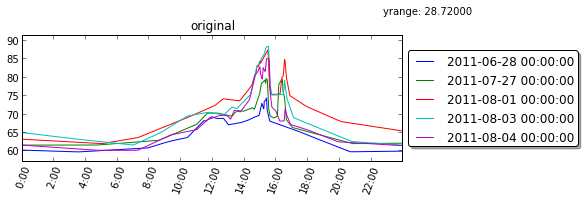
\includegraphics[width=8cm]{fig-original}
  \caption{Original sensor values}
  \label{fig:results-original}
\end{subfigure}%
\begin{subfigure}{8cm}
  \centering
  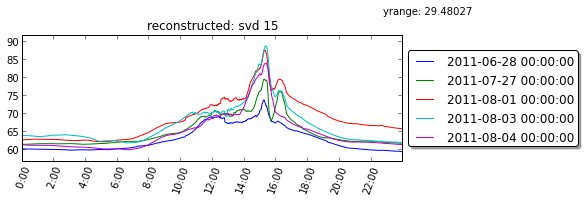
\includegraphics[width=8cm]{fig-reconstructed_svd}
  \caption{Reconstructed sensor values from SVD model}
  \label{fig:results-reconstructed-svd}
\end{subfigure}
\caption{Measurements from a single sensor for 5 days}
\label{fig:results}
\end{figure}

\newpage


\end{document}

